%---------------------------------------------------------------------
\begin{frame}{}

    It is pre-ACA. You are 30 years old, and do not qualify for Medicaid.
    You new employer does not offer healthcare insurance plans.
    You would really value getting health insurance, because you are risk-averse and because you know the cost of healthcare is extremely high if you get sick.\\
    \vspace{5mm}

    How would you get health insurance?\\
    \vspace{5mm}
    \pause
    $\implies$ You would get a quote on an insurer's website. For example: \href{https://www.cignaglobal.com/quote}{Cigna quote}.\\
    \pause

    Well, just like the market for pet insurance today! For example: \href{https://www.healthypawspetinsurance.com}{Healthy Paws pet insurance}.\\
    
\end{frame}
%---------------------------------------------------------------------
\begin{frame}{Pre-ACA individual insurance market}

    Buying insurance on the individual market used to be difficult.
    \begin{itemize}
        \item Detailed medical underwriting
        \item Questions about personal and family health history
        \item Higher premiums for risky applicants
        \item Sometimes outright denial of coverage
        \item Sometimes exclusions for specific conditions
    \end{itemize}

    \vspace{3mm}

    Insurers tried to protect themselves from high expected costs.

\end{frame}
%---------------------------------------------------------------------
\begin{frame}{Why did the ACA matter?}

    Video: \href{https://www.youtube.com/watch?v=P9LTAageny0}{``The story of the Affordable Care Act''}

\end{frame}
%---------------------------------------------------------------------
\begin{frame}{}

    \begin{center}
        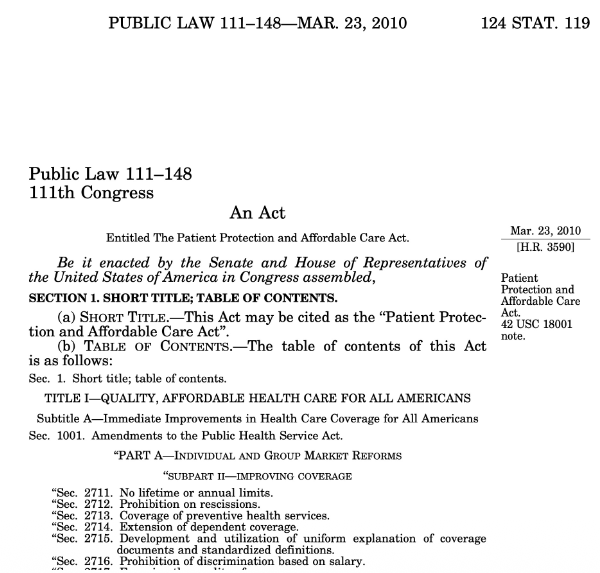
\includegraphics[width=0.6\textwidth]{input/ACA_front.png}
    \end{center}
    \vspace{-3mm}

    Link to full law \href{https://www.govinfo.gov/content/pkg/PLAW-111publ148/pdf/PLAW-111publ148.pdf}{here}.
    
\end{frame}
%---------------------------------------------------------------------
\begin{frame}{Why did the ACA matter?}

    Before the ACA, about \newbold{50 million Americans} lacked health insurance.
    \begin{itemize}
        \item Some were young and healthy and chose to remain uninsured
        \item Others had jobs without coverage
        \item Others had \newbold{pre-existing conditions} that made private coverage expensive or unavailable
    \end{itemize}

    \vspace{3mm}

    The ACA kept the U.S. patchwork system, but it \newbold{dramatically reformed} the individual insurance market.

\end{frame}
%---------------------------------------------------------------------
\begin{frame}{Sources of health insurance coverage \newbold{2023}}
    \vspace{-1mm}
    \begin{center}
        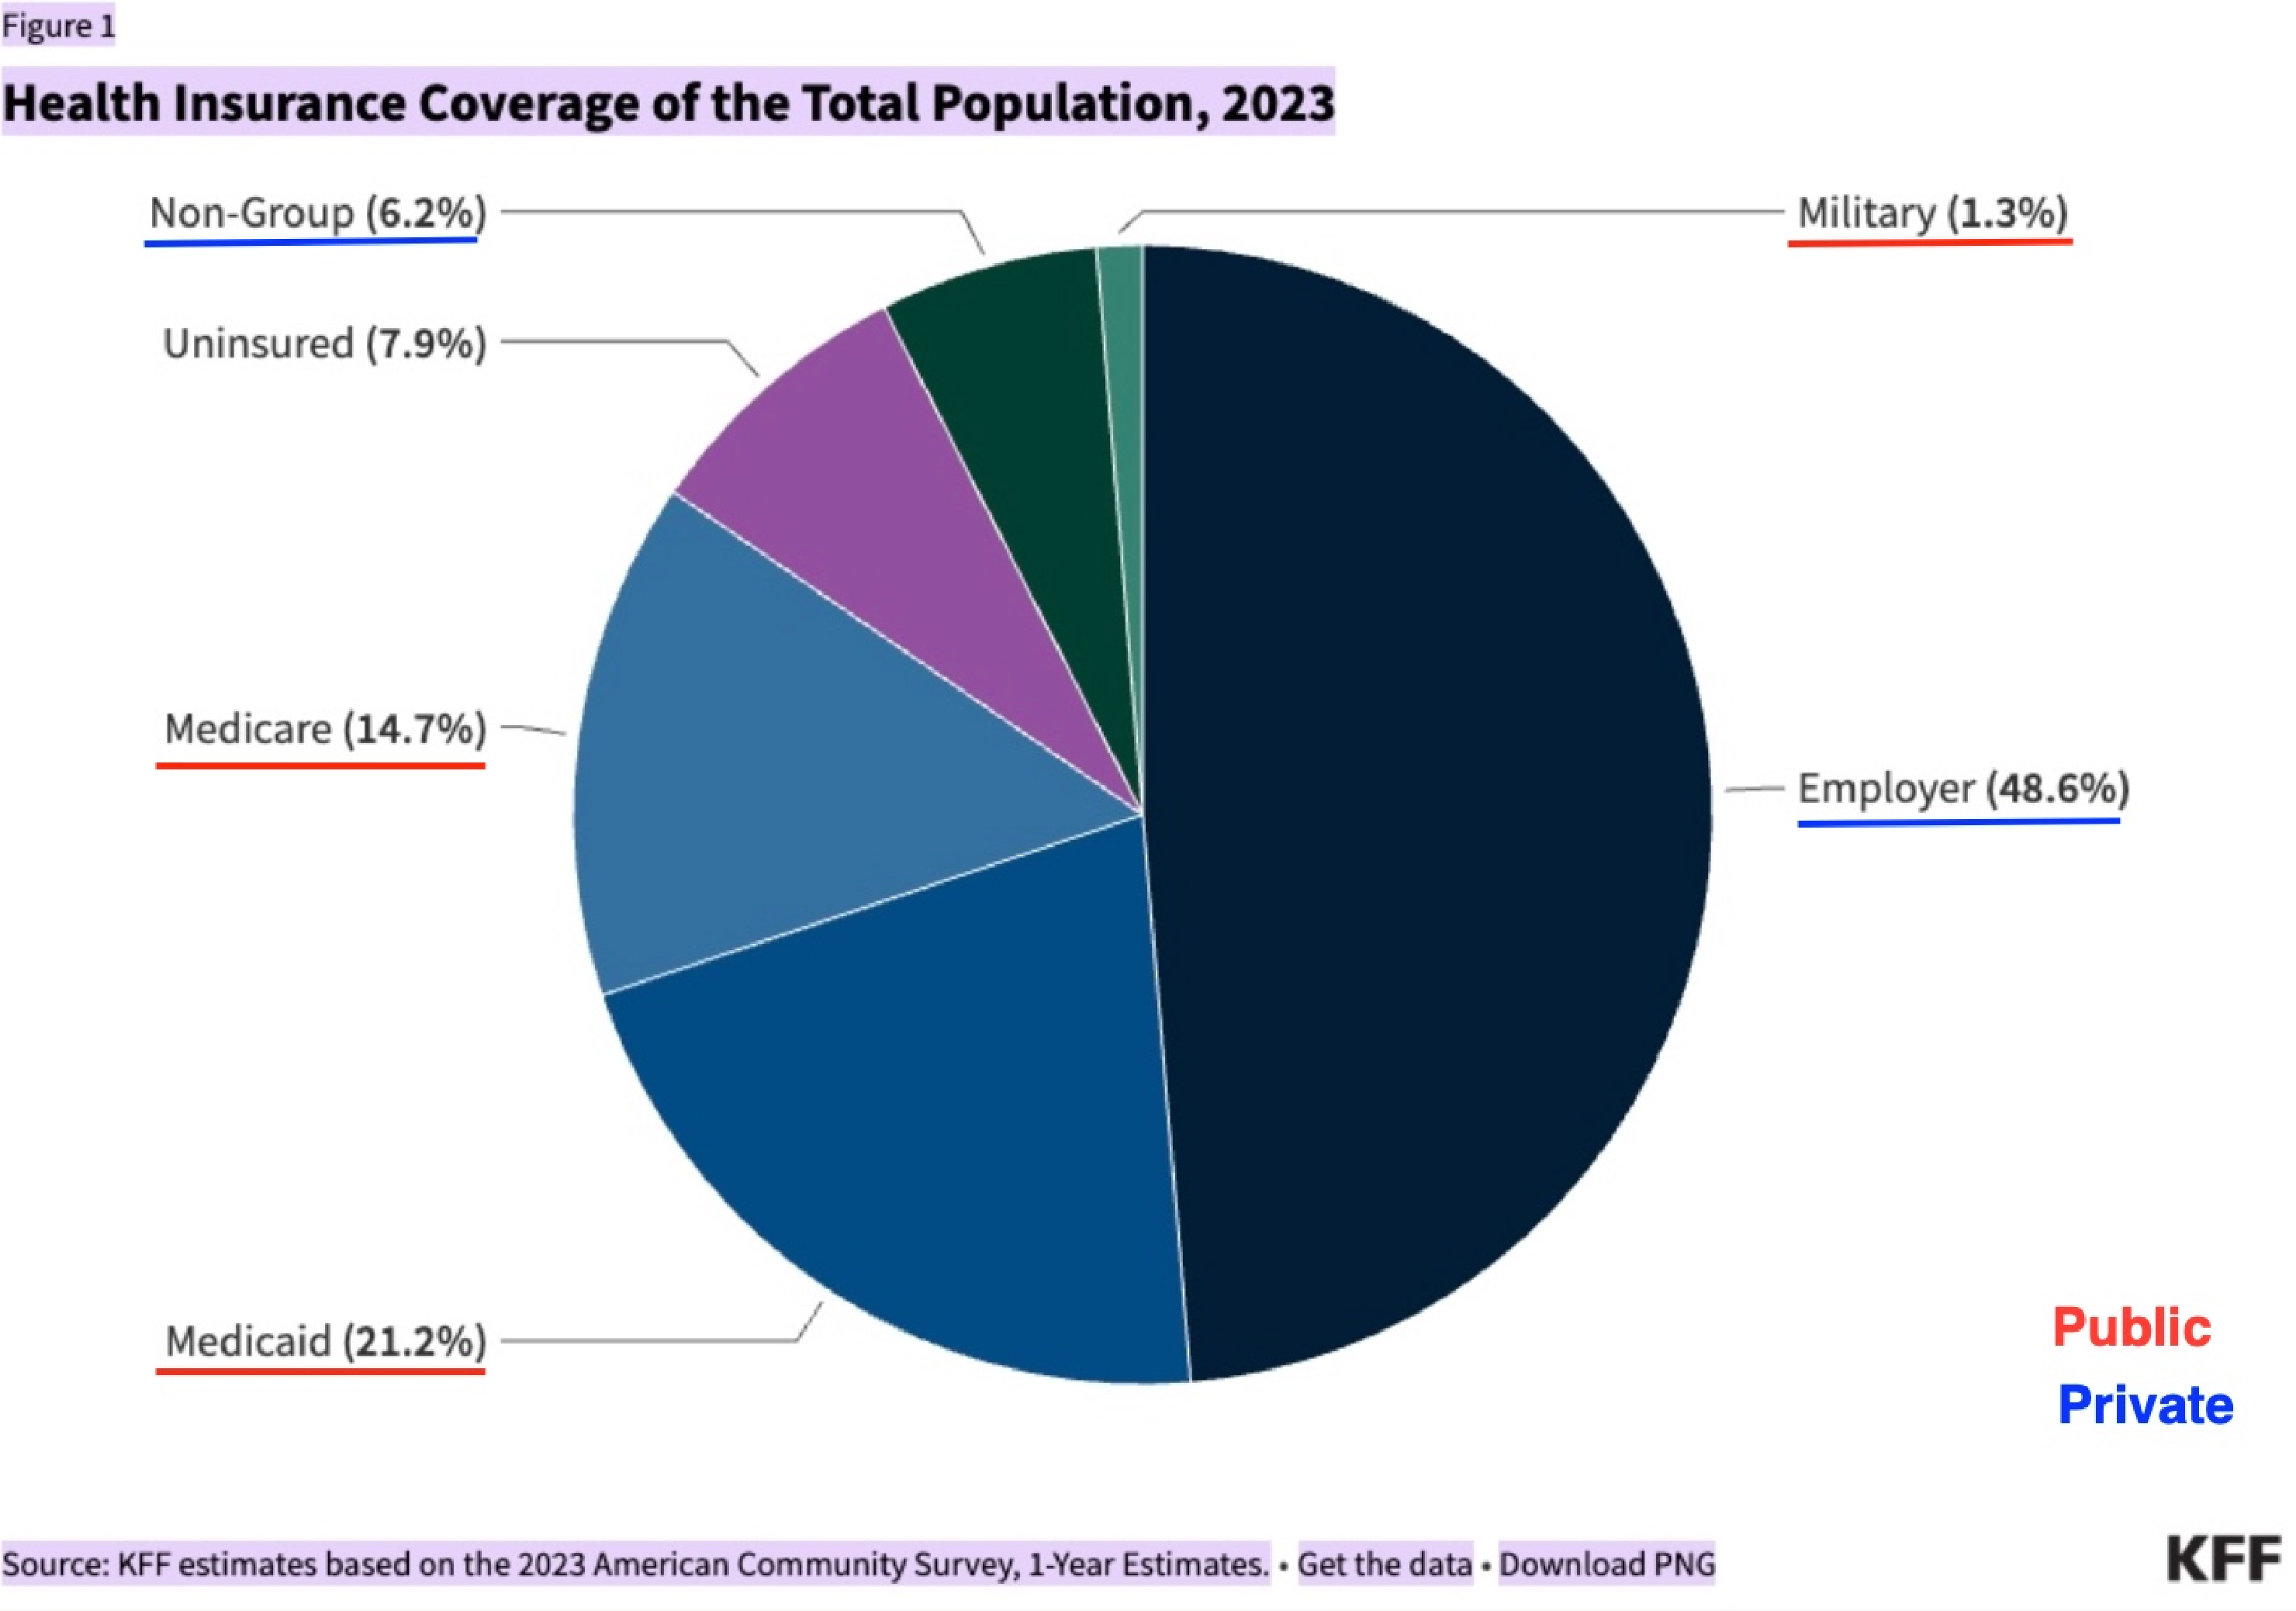
\includegraphics[height=0.85\textheight]{input/KFF_healthinsurancecoverage2023_highlights.pdf}
    \end{center}
\vspace{-5mm}

{\tiny Source: \href{https://www.kff.org/uninsured/health-policy-101-the-uninsured-population-and-health-coverage/?entry=table-of-contents-who-is-uninsured-in-the-united-states}{KFF website}.}
\end{frame}
%---------------------------------------------------------------------
\begin{frame}{The ACA as a ``three-legged stool''}

    The ACA as a \newbold{three-legged stool} (Jonathan Gruber):
    \begin{enumerate}
        \item \newbold{Regulation} of the individual market
        \item An \newbold{individual mandate}
        \item Policies making insurance \newbold{more affordable}
    \end{enumerate}

    \vspace{3mm}

    Logic:
    \begin{itemize}
        \item Regulation alone risks adverse selection
        \item A mandate alone is regressive
        \item Subsidies make broad participation politically and financially feasible
    \end{itemize}

\end{frame}
%---------------------------------------------------------------------
\begin{frame}{Guaranteed issue and community rating}

    The ACA sharply restricted insurer pricing.
    \begin{itemize}
        \item Premiums can vary only by \newbold{location, age, and tobacco use}
        \item Insurers can no longer price on most health risks
        \item Insurers cannot refuse customers because of \newbold{pre-existing conditions}
    \end{itemize}

    \vspace{3mm}

    This is \newbold{guaranteed issue} plus \newbold{community rating}: people in the same local market face the same menu of plans.

\end{frame}
%---------------------------------------------------------------------
\begin{frame}{Who gains and who loses from community rating?}

    Community rating redistributes across risk types.
    \begin{itemize}
        \item \newbold{Sicker people gain}: they can buy coverage at much better terms
        \item \newbold{Healthier people lose}: they no longer get especially cheap, customized prices
        \item Reclassification risk falls for everyone: if you become sick, you cannot be priced out later
    \end{itemize}

    \vspace{3mm}

    So the ACA trades off:
    \begin{itemize}
        \item Less pricing based on risk
        \item More pooling across healthy and sick consumers
    \end{itemize}

\end{frame}
%---------------------------------------------------------------------
\begin{frame}{Essential health benefits: minimum benefit requirements}

    The ACA also regulates \newbold{what plans must cover}.
    \begin{itemize}
        \item Required to cover services in \href{https://www.healthcare.gov/coverage/what-marketplace-plans-cover/}{10 categories of essential health benefits}
        {\footnotesize {\color{gray} (example: emergency services hospitalization, maternity care, mental health, pediatric services, etc.)}}
        % \item Emergency services
        % \item Hospitalization
        % \item Maternity and newborn care
        % \item Mental health and substance use treatment
        % \item Prescription drugs
        % \item Rehabilitation services
        % \item Laboratory services
        % \item Preventive care
        % \item Pediatric services

        \item Preventive and wellness services must be covered \newbold{with no cost-sharing}
    \end{itemize}
    \vspace{5mm}

    The ACA also regulates \newbold{how much plans must cover} in terms of actuarial value
    \begin{align*}
            \text{actuarial value} = \frac{\text{average expenses paid by insurer}}{\text{average total health care expenses}} > 0.6
    \end{align*}
\end{frame}
%---------------------------------------------------------------------
\begin{frame}{Metal tiers and actuarial value}

    \begin{center}
        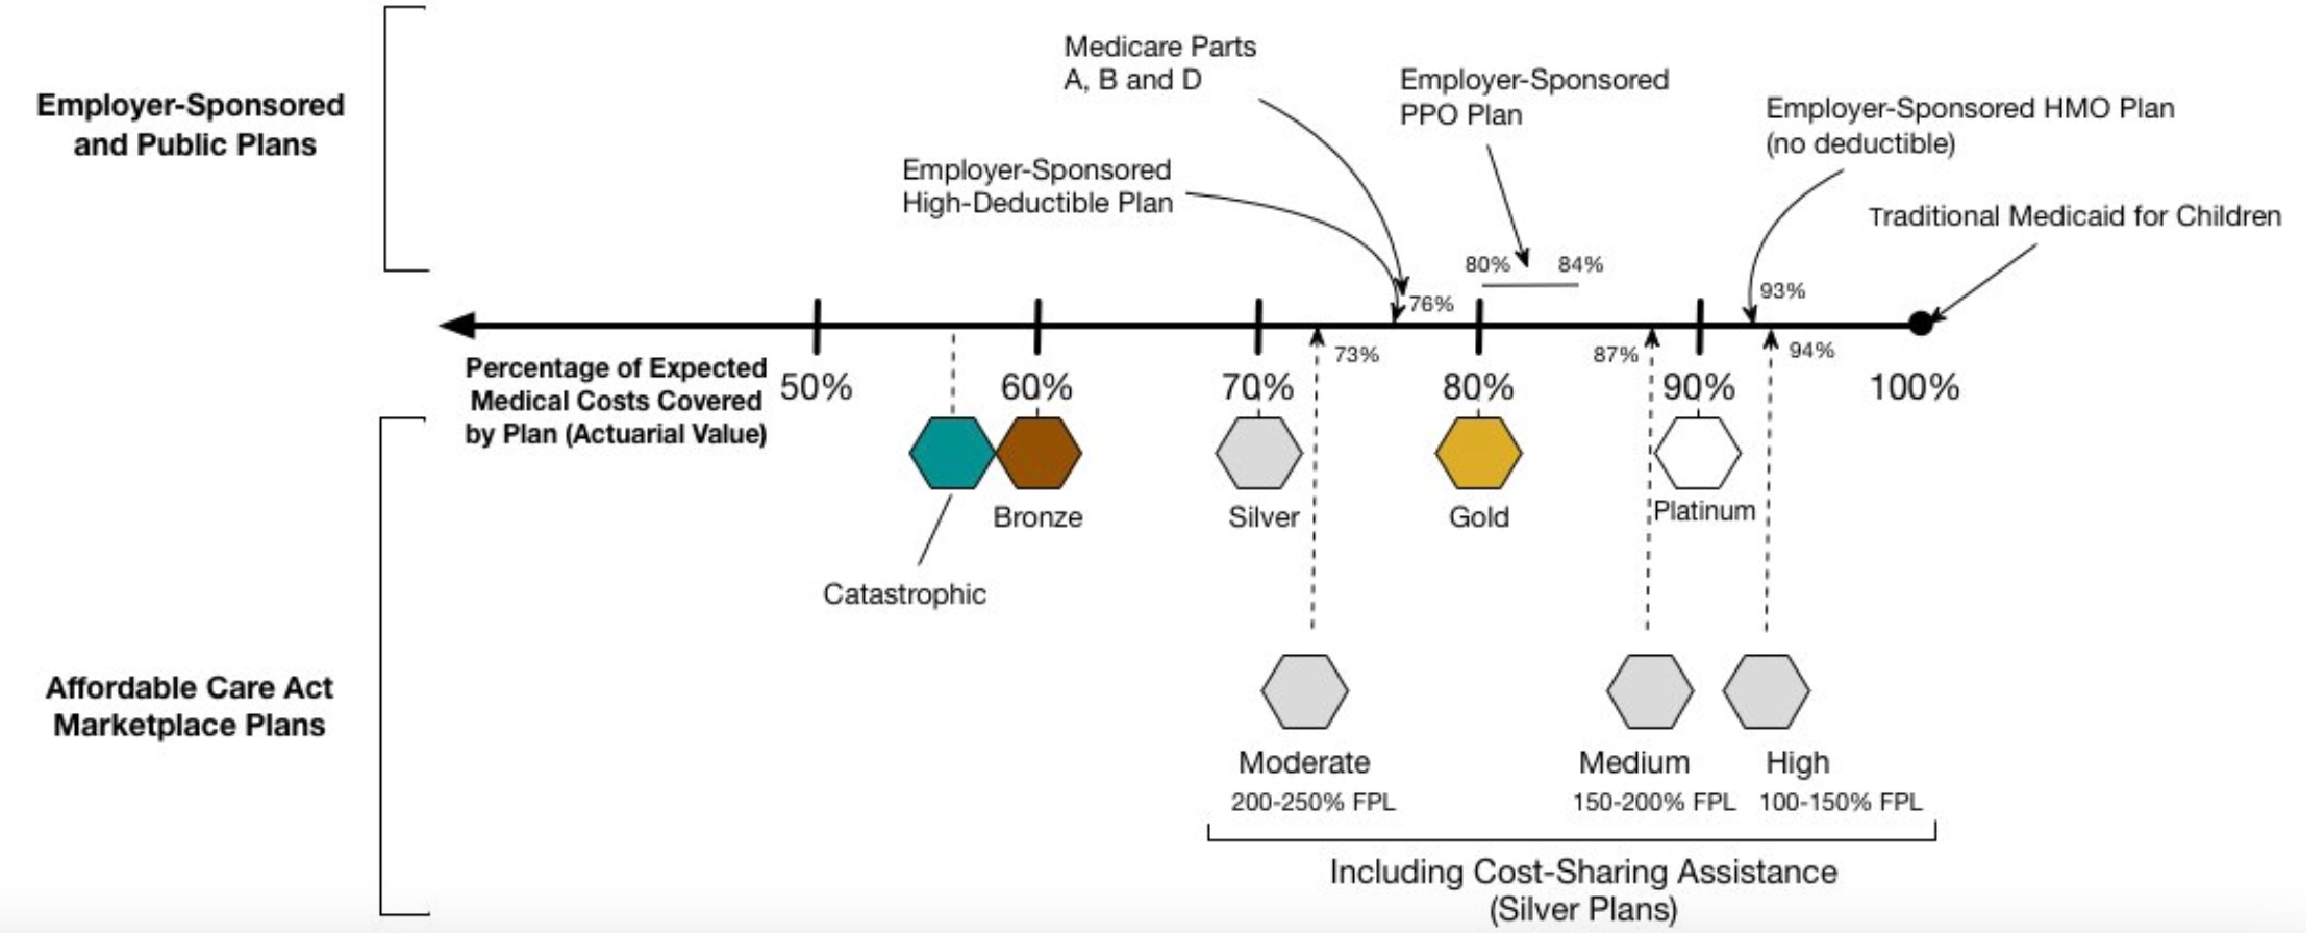
\includegraphics[width=0.8\textwidth]{input/plans_coverage_ratings.pdf}
    \end{center}

    Plans below roughly \newbold{60\% actuarial value} are generally not allowed on the marketplace.

\end{frame}
%---------------------------------------------------------------------
\begin{frame}{Other insurance regulations}

    The ACA also removed some older forms of weak coverage
    \begin{itemize}
        \item Ban on \newbold{lifetime spending limits}
        \item More standardization of plan generosity
        \item More transparency when comparing policies
    \end{itemize}

    \vspace{3mm}

    Idea:
    \begin{itemize}
        \item Insurance should be available
        \item Insurance should be meaningful when people get sick
    \end{itemize}

\end{frame}
%---------------------------------------------------------------------
\begin{frame}{What are the Individual Marketplaces?}

    \newbold{For whom?} For people who do not have employer-sponsored insurance, Medicare, or Medicaid.\\
    \vspace{5mm}

    \newbold{What is it?} A ``place'' to shop for insurance.\\
    For most states: \href{https://www.healthcare.gov/}{healthcare.gov} is the marketplace.
    \begin{itemize}
        \item Health insurance plans must comply with the rules of the ACA
        \item Information is provided in a standardized way to facilitate comparison
        \item Subsidies are available for purchasers with income below 400\% of the federal poverty level (FPL)
    \end{itemize}
\end{frame}
%---------------------------------------------------------------------
\begin{frame}{Why an individual mandate?}

    Once insurers must cover everyone, a new problem appears:
    \begin{itemize}
        \item Why not wait until you get sick to buy insurance?
    \end{itemize}

    \vspace{3mm}

    If only sick people enroll:
    \begin{itemize}
        \item average costs rise
        \item premiums rise
        \item healthy people leave
        \item the market can unravel
    \end{itemize}

    The \newbold{individual mandate} was meant to keep healthy people in the risk pool.

\end{frame}
%---------------------------------------------------------------------
\begin{frame}{How strong was the mandate?}

    The penalty phased in over time.

    \begin{center}
    \begin{tabular}{lcc}
        \toprule
        Year & Flat fee & Share of income \\
        \midrule
        2014 & \$95 & 1.0\% \\
        2015 & \$325 & 2.0\% \\
        2016 & \$695 & 2.5\% \\
        \bottomrule
    \end{tabular}
    \end{center}

    \vspace{2mm}

    Problem:
    \begin{itemize}
        \item The penalty was often much lower than the premium for insurance
        \item Some healthy consumers preferred to stay uninsured and pay the penalty
    \end{itemize}

\end{frame}
%---------------------------------------------------------------------
\begin{frame}{Why the mandate may have been weak}

    Why the mandate may not have been strong enough to fully stabilize the market:
    \begin{itemize}
        \item Around \newbold{6.5 million taxpayers} paid the penalty in 2015
        \item Average penalty was only about \newbold{\$470}
        \item Some consumers enrolled, used care, and dropped coverage soon after
    \end{itemize}

    \vspace{3mm}

    Later, the 2017 tax law reduced the federal penalty to \newbold{zero starting in 2019}.

\end{frame}
%---------------------------------------------------------------------
\begin{frame}{The employer mandate}

    The ACA also includes an \newbold{employer mandate}.
    \begin{itemize}
        \item Firms with more than 50 employees are required to offer employer-sponsored insurance
    \end{itemize}

    \vspace{3mm}

    Why this matters:
    \begin{itemize}
        \item Most Americans get coverage through employers
        \item The ACA was not trying to replace employer insurance
        \item It mostly targeted gaps in the individual and Medicaid markets
    \end{itemize}

\end{frame}
%---------------------------------------------------------------------
\begin{frame}{Affordability was the central problem}

    In 2016, the average annual premium for a Silver plan was about \newbold{\$4,583} for one person.

    \vspace{3mm}

    Compare that to the 2016 federal poverty level for an individual:
    \begin{itemize}
        \item \newbold{\$11,770}
    \end{itemize}

    \vspace{3mm}

    Without subsidies, insurance would absorb a huge share of income for poor households.

\end{frame}
%---------------------------------------------------------------------
\begin{frame}{How subsidies work?}

    For whom?
    \begin{enumerate}
        \item People buying a plan on the Individual Marketplace
        % If employer-sponsored you don't get it, Medicaid you don't need it
        \item If you are below 400\% of the federal poverty level (FPL)
        \begin{itemize}
            \item Exact amount depends on a complex formula that includes income
            \item Tied to second-lowest-cost plan in your area
            % If premium increase you are protected
            % For subsidy-eligible households, premium increases do not fully translate into higher out-of-pocket premiums
        \end{itemize}
    \end{enumerate}
    \vspace{3mm}

    How what it given to people? \newbold{Advanced tax credit}
    \begin{itemize}
        \item Choose a plan in 2021: forecast your subsidy based on 2020 income
        \item The government pays the subsidy directly to the insurer using 2020 income
        \item April 2022: reconciliation depending on your actual 2021 income
    \end{itemize}

\end{frame}
%---------------------------------------------------------------------
\begin{frame}{Federal poverty level}

   \begin{center}
    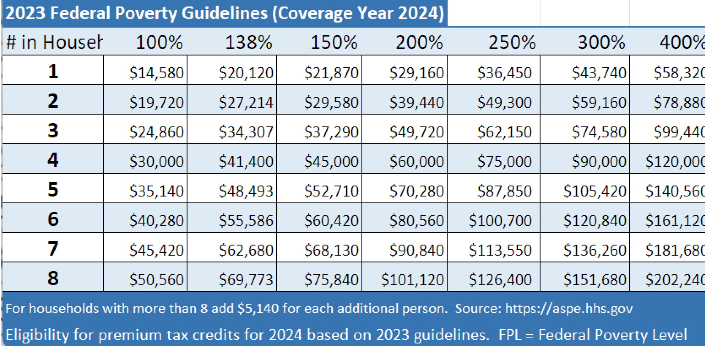
\includegraphics[width=0.8\textwidth]{input/FPL_2023.png}
    \end{center}

    \begin{minipage}{\textwidth}
    \scriptsize
    \renewcommand{\baselinestretch}{1}\selectfont
    Defines the income level which is considered to be ``living in poverty''.
    Where does it come from? Someone came up with it about 60 years ago (1963), and indexed it to inflation since then.
    The Johnson administration adopted it, and it has been a fixture in federal regulations ever since.
    \end{minipage}
\end{frame}
%---------------------------------------------------------------------
\begin{frame}{How exactly do they work? Go check it out}

    KFF Health Insurance Marketplace Calculator: \href{https://www.kff.org/interactive/subsidy-calculator/}{https://www.kff.org/interactive/subsidy-calculator/}

\end{frame}
%---------------------------------------------------------------------
\begin{frame}{Cost-sharing reductions}

    The ACA also subsidized \newbold{deductibles, copays, and other cost sharing} for lower-income buyers.

    \begin{center}
    \begin{tabular}{lc}
        \toprule
        Income level & After-subsidy actuarial value \\
        \midrule
        150\% FPL & 94\% \\
        200\% FPL & 87\% \\
        250\% FPL & 73\% \\
        400\% FPL & 70\% \\
        \bottomrule
    \end{tabular}
    \end{center}

    \vspace{2mm}

    So the ACA tried to reduce both:
    \begin{itemize}
        \item premiums
        \item out-of-pocket exposure
    \end{itemize}

\end{frame}
%---------------------------------------------------------------------
\begin{frame}{The supply side problem}

    The ACA did not just need buyers.
    \begin{itemize}
        \item It also needed insurers willing to offer plans on the exchanges
    \end{itemize}

    \vspace{3mm}

    Why insurers were nervous:
    \begin{itemize}
        \item They could no longer finely price risk
        \item They did not know exactly who would enroll
        \item Costs depend on the health of the people who sign up
    \end{itemize}

    \vspace{3mm}

    The transition to the new system created a lot of uncertainty.

\end{frame}
%---------------------------------------------------------------------
\begin{frame}{The ``3Rs'' for insurers}

    To stabilize insurer participation, the ACA created the \newbold{3Rs}:
    \begin{enumerate}
        \item \newbold{Risk-adjustment}
        \item \newbold{Reinsurance}
        \item \newbold{Risk corridors}
    \end{enumerate}

    \vspace{3mm}

    Goal:
    \begin{itemize}
        \item protect insurers from unexpectedly sick pools
        \item reduce incentives for cream-skimming
        \item encourage insurer entry into new marketplaces
    \end{itemize}

\end{frame}
%---------------------------------------------------------------------
\begin{frame}{Risk adjustment}

    Risk adjustment was designed as the \newbold{permanent} stabilization policy.

    \begin{itemize}
        \item Insurers submit demographic and diagnostic data
        \item Government computes a risk score
        \item Plans with healthier enrollees transfer money to plans with sicker enrollees
    \end{itemize}

    \vspace{3mm}

    If calibrated well, risk adjustment reduces incentives to avoid sick customers.

\end{frame}
%---------------------------------------------------------------------
\begin{frame}{Reinsurance and risk corridors}

    These were \newbold{temporary} transition policies.

    \begin{itemize}
        \item \newbold{Reinsurance}: government helps cover very high-cost enrollees
        \item \newbold{Risk corridors}: insurers with unusually high losses receive support, financed partly by insurers with unusually high gains
    \end{itemize}

    \vspace{3mm}

    Both were meant to make the early ACA years less risky for insurers.

\end{frame}
%---------------------------------------------------------------------
% \begin{frame}{Implementation problems with the 3Rs}

%     In practice, these programs were not fully funded relative to realized claims.

%     \begin{itemize}
%         \item 2015 reinsurance contributions: about \newbold{\$6.5 billion}
%         \item 2015 reinsurance requests: about \newbold{\$14.3 billion}
%         \item 2014 risk corridor collections: about \newbold{\$0.36 billion}
%         \item 2014 risk corridor claims: about \newbold{\$2.87 billion}
%     \end{itemize}

%     \vspace{3mm}

%     This contributed to insurer exits, lawsuits, and continued instability.

% \end{frame}
%---------------------------------------------------------------------
\begin{frame}{Medicaid expansion}

    The ACA expanded Medicaid to adults under 65 with income up to about \newbold{133\% of the federal poverty level}.\\
    \textit{Reminder: Medicaid is a \newbold{means-tested} program, meaning you must qualify for it based on your
    ``means'' (a combination of income, assets, employment status, demographics, and
    household composition)}

    \begin{itemize}
        \item Before the ACA, state Medicaid rules varied enormously
        \item Some states were generous
        \item Others barely covered poor parents and often excluded childless adults
    \end{itemize}

    \vspace{3mm}

    Federal government financing was initially very generous, eventually settling at \newbold{90\%} for the newly eligible.

\end{frame}
%---------------------------------------------------------------------
\begin{frame}{Why Medicaid expansion became uneven}

    In \newbold{NFIB v. Sebelius (2012)}, the Supreme Court ruled that states could not be forced to expand Medicaid.

    \vspace{3mm}

    Result:
    \begin{itemize}
        \item Medicaid expansion became \newbold{optional}
        \item Some states expanded quickly
        \item Others did not
    \end{itemize}

    \vspace{3mm}

    This matters for marketplace premiums too:
    \begin{itemize}
        \item Without expansion, poorer and often sicker people remain in the private market
    \end{itemize}

\end{frame}
%---------------------------------------------------------------------
\begin{frame}{Why Medicaid expansion became uneven}

\begin{center}
    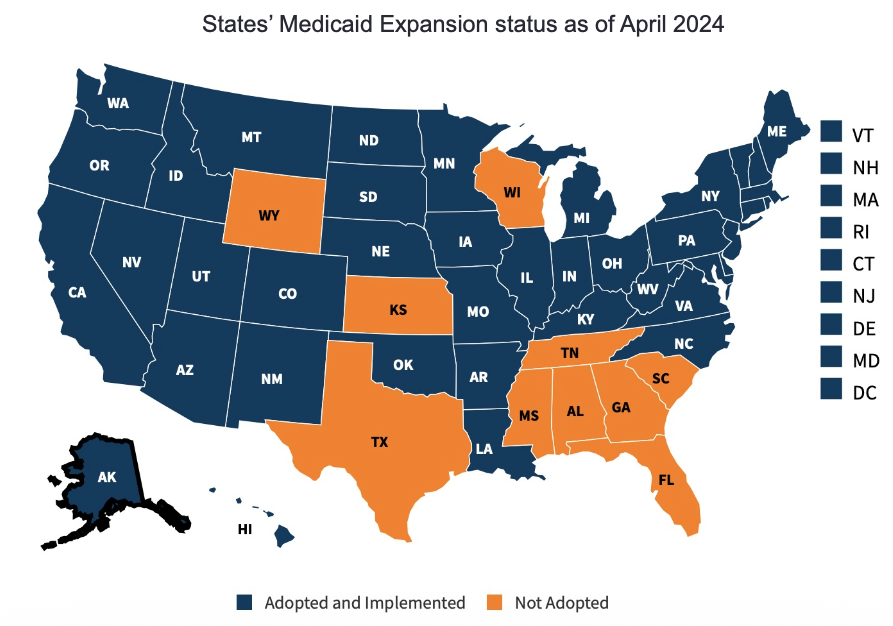
\includegraphics[width=0.75\textwidth]{input/map_Medicaidexpansions2024.png}
\end{center}
\end{frame}
%---------------------------------------------------------------------
\begin{frame}{A gap...}

\begin{center}
    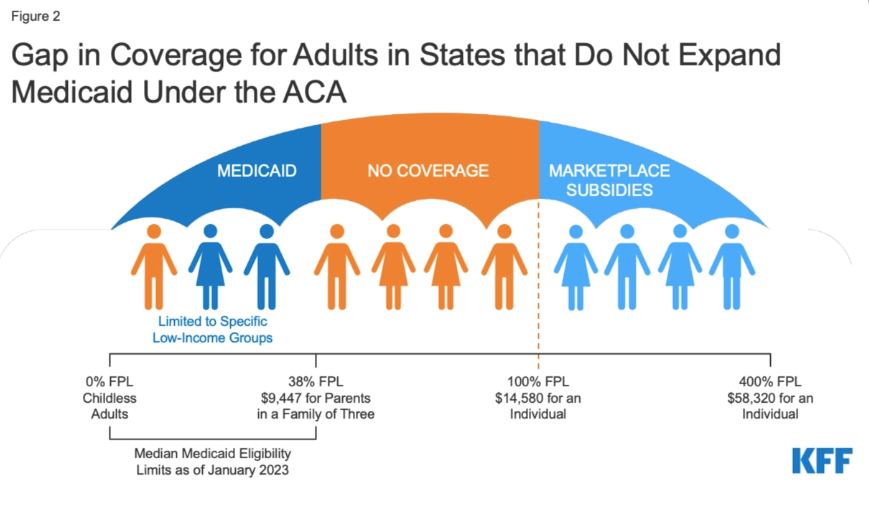
\includegraphics[width=0.8\textwidth]{input/Medicaid_gap.png}
\end{center}
\end{frame}
%---------------------------------------------------------------------
% \begin{frame}{}

% \begin{center}
%     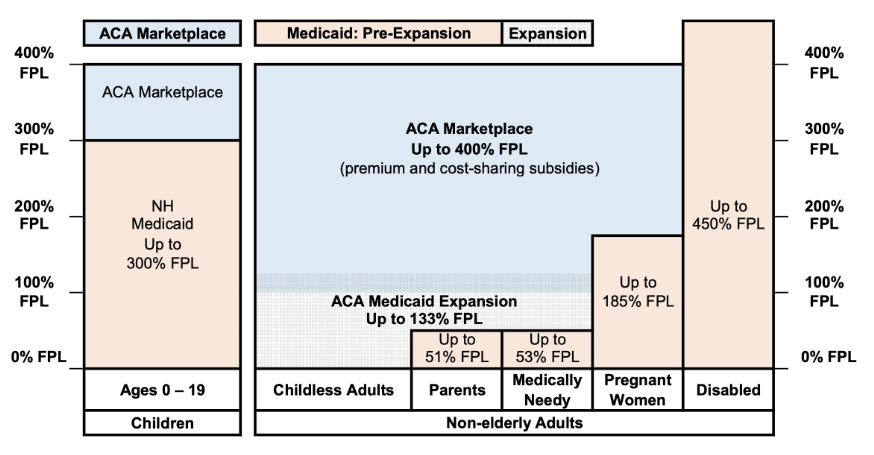
\includegraphics[width=0.8\textwidth]{input/exampleNH.png}
% \end{center}

% Example from New Hampshire, but similar in most states.
% \end{frame}
%---------------------------------------------------------------------
\begin{frame}{How was the ACA financed?}

    Coverage expansion was expensive.

    \begin{itemize}
        \item Medicaid expansion
        \item Premium subsidies
        \item Cost-sharing subsidies
        \item Marketplace stabilization programs
    \end{itemize}

    \vspace{3mm}

    Examples
    \begin{itemize}
        \item Medicare and Medicaid cost-control measures
        \item Higher taxes on high-income households
        \item New taxes on some sectors and products
        \item The planned ``Cadillac tax'' on very generous plans (never implemented)
    \end{itemize}

\end{frame}
%---------------------------------------------------------------------
\begin{frame}{Effect of the ACA?}

   \begin{center}
    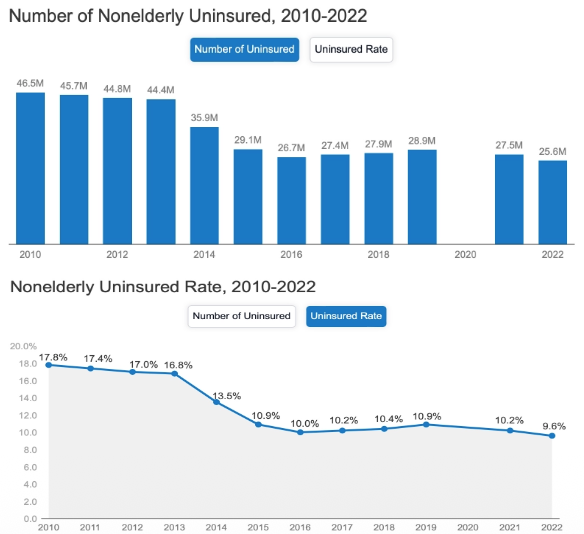
\includegraphics[width=0.5\textwidth]{input/uninsured_graphs.png}
    \end{center}
    \pause
    \vspace{-3mm}

    \newbold{More details next week.}

    {\tiny Source: \href{https://www.kff.org/uninsured/key-facts-about-the-uninsured-population/}{KFF website}.}

\end{frame}
%---------------------------------------------------------------------
\begin{frame}{The ACA today}

    \begin{itemize}
        \item Dozens of unsuccessful full repeal attempts
        \item Repeal of individual mandate in 2017 (set penalty to zero)
        \item Coverage gap for individuals in non-expansion states remains
        \item First Trump administration also ended
        \begin{itemize}
            \item Cost-sharing subsidies
            \item Allowed short-term (``skinny'' or ``short-term''), non-compliant plans. Cheap but no subsidy
            \item Funds supporting healthcare.gov reduced
        \end{itemize}
        \item Biden administration has reversed many of these changes, but then reversed again
    \end{itemize}

    $\implies$ \newbold{The core ACA structure (exchanges, Medicaid expansion, guaranteed issue) is still in place}

\end{frame}
%---------------------------------------------------------------------
% \begin{frame}{Why the ACA stayed politically fragile}

%     The chapter's discussion of the ACA is also a lesson in political economy.

%     \begin{itemize}
%         \item It expanded coverage, but through a complex hybrid system
%         \item Different pieces depended on one another
%         \item Court decisions, administrative choices, and congressional funding fights weakened several legs of the stool
%     \end{itemize}

%     \vspace{3mm}

%     So even when the ACA survived formal repeal, it still faced partial erosion.

% \end{frame}
%---------------------------------------------------------------------
\begin{frame}{Takeaways}

    Three main ``legs'' of the ACA:
    \begin{enumerate}
        \item \newbold{Regulation} of the individual market
        \item An \newbold{individual mandate}
        \item Policies making insurance \newbold{more affordable}
    \end{enumerate}
    \vspace{3mm}

    Political economy of the ACA:
    \begin{itemize}
        \item It expanded coverage, but through a complex hybrid system
        \item Different pieces depended on one another
        \item Court decisions, administrative choices, and congressional funding fights weakened several legs of the stool
    \end{itemize}

    % \begin{enumerate}
    %     \item The ACA aimed to solve both \newbold{access} and \newbold{adverse selection}
    %     \item Its logic depended on combining regulation, mandates, and subsidies
    %     % \item Medicaid expansion and subsidies were central to increasing coverage
    %     % \item The individual mandate may have been too weak to fully stabilize risk pools
    %     % \item The ACA improved financial protection, but marketplace stability remained a challenge
    % \end{enumerate}

\end{frame}
%---------------------------------------------------------------------
\begin{frame}{}
    \begin{center}
    \Large \textcolor{maroon}{Wrapping up}
    \end{center}
\end{frame}
%---------------------------------------------------------------------
\begin{frame}{To next class}
\begin{itemize}
    \item \newbold{TO DO}
    \begin{enumerate}
        \item \newbold{Problem set 4} posted: due \newbold{Thursday March 26th by 9:30am}
        \item Review this class and past material $\implies$ \textit{questions on it?}
    \end{enumerate}
    \vspace{5mm}

    \item Program for next class
    \begin{itemize}
        \item Impact of the ACA
        \item Who remains uninsured?
    \end{itemize}
\end{itemize}
\end{frame}
%---------------------------------------------------------------------